% It is an example file showing how to use the 'acm_proc_article-sp.cls' V3.2SP
% LaTeX2e document class file for Conference Proceedings submissions.
\documentclass{edm_template}


\usepackage{amsmath}
\usepackage{graphics}

% Somehow the desired top margin is being set to 1/16in?
\addtolength{\topmargin}{0.6875in}

\begin{document}

% Title portion
\title{Self-improving intelligent tutor system}
\numberofauthors{1}
\author{
\alignauthor
      Brett van de Sande\\
       \affaddr{Arizona State University}\\
       \affaddr{PO Box 878809}\\
       \affaddr{Tempe, AZ~~85287}\\
       \email{bvds@asu.edu}
}
\maketitle

% Assignment of blame paper: 
% http://www.public.asu.edu/~kvanlehn/Stringent/PDF/07UM_KVL_KK_etal.pdf
%   my ``opportunity'' equals their ``step''
%   my ``turn'' equals their ``transaction''
%
% Doing reinforcement learning by direct policy search.
% See discussion on p. 17 of:
% http://www.cs.brown.edu/research/pubs/theses/phd/2002/peshkin.pdf



\begin{abstract}
Human tutors constantly make decisions about
what kind of help they are going to give (or not give).  Ideally,
they make these decisions based on some determination of how
the student is progressing coupled with some knowledge of what kind
of tutoring strategies have worked in similar situations in the past.
Computer tutors, in contrast, often have fixed policies for their
tutoring strategies.   Can we do better?  To address this question, 
we have implemented a method for iteratively improving 
help-giving policies of a computer tutor for introductory physics.  
We created a version of the tutor that randomly uses one of several 
(reasonable) policies when helping students and deployed it in the
classroom.  We then used the resulting student log data to 
train a new version of the tutor having improved hinting policies
and deployed the new version of the tutor in the classroom.  
We discuss what is needed to make this into a sustainable iterative process.
\end{abstract}

\keywords{data mininig, models of student learning}

\section{Introduction}


Intelligent tutor systems (ITS) have become increasingly sophisticated
over the years.  Interaction with the students is slowly evolving
from multiple-choice input with static feedback [OLI? CTAT] to more 
sophisticated forms of interaction.  Now days, one can find systems with 
free-form drawing interfaces [Andes], and interactive dialogs [cite Grasser,
Cordillera, etc.].  Along with the more sophisticated interactions
with the student, comes a larger, more complicated set of 
decisions the ITS must make, for example:
%
\label{intro}
\begin{itemize}

   \item Do I tell the student what to do next or remain silent?

   \item Do I give a hint or wait until the student asks?

   \item Do I give a pointing hint or do I tell the student 
         what to do next, explicitly?

   \item Did the student really learn how to do this or should
         I suggest more practice?

   \item Do I show them a video, or do I just tell them something?
         Should I put up a modal dialog box, so they can't miss the
         help given?

   \item Should I ask the student a question to determine their 
         current affect/understanding?

\end{itemize}

Theories of learning can tell us what kind of help-giving
strategies may be effective and, broadly, when they might be effective.
Likewise, theories of learning may help us identify what kinds of 
features might be useful for determining the student's ``state'' at
a given moment.  The purpose of this project is to fill in the gap
by determining exactly what help-giving strategy the tutor should use for a 
particular student state.
The task of finding an optimal help-giving strategy for a
given student state is commonly known as 
Reinforcement Learning~\cite{kaelbling_reinforcement_1996}.
We use past student behavior in response to various help-giving
actions on the part of the tutor to construct a reward function
and use that reward function to determine an optimal hinting policy.
We will use a direct policy search strategy for determining the optimal
policy~\cite{rosenstein_robot_2001}.

Since the agent must give hints in real time, the student state
must contain features that are available in real time, so that
the learned policy can be applied immediately.  In contrast,
the reward function uses subsequent student actions and is only
available after the fact.  Thus, there must be a two-phase process:
an {\em off-line learning phase'} to determine the optimal help-giving 
policy and an {\em online tutoring phase'} where the policy is applied.
This leads to an iterative process where one alternates between 
the {\em off-line learning phase} and the {\em online tutoring phase}.

\section{Improvment Process}
%
%  The diagram was created by process.odg
%  In CentOS, eps exporting in OpenOffice has problems with 
%  creating bounding boxes.  The following process worked:
%  1.  in draw, select the entire diagram
%  2.  in draw, export pdf, choosing 'selection' as source
%      with file name process.pdf
%  3.  pdf2ps process.pdf 
%  4.  mv process.ps process.eps
%  5.  rm process.pdf
%
% On OS X 10.8, Open Office 3.4.1, the export to eps works fine.
%
\begin{figure*}
\centering    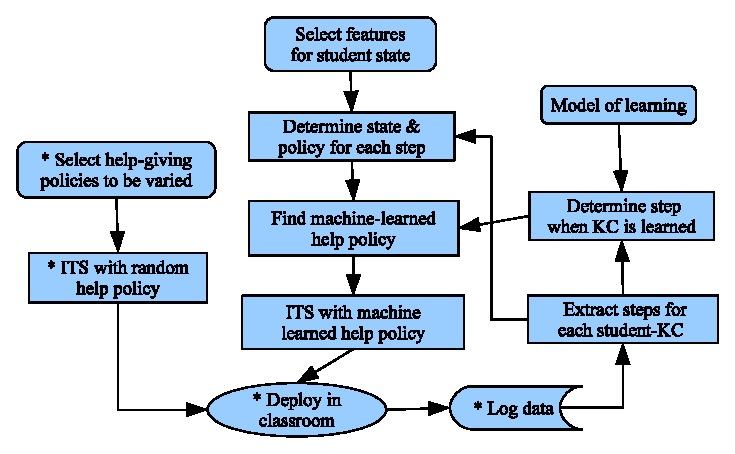
\includegraphics{process.eps}
\caption{Iterative process for improvement of help-giving policies in
  an intelligent  tutor system (ITS).  The steps corresponding to Study 1 are marked
  with an asterisk.} \label{process}
\end{figure*}

Let us describe this process in more detail; see Fig.~\ref{process}.  The first
step is to identify a set of tutoring policies that can be varied,
such as those listed in Section~\ref{intro}.  Since we have no {\em a priori}
way of choosing what policy is optimal, we create a version of the ITS
that randomly chooses between the possible help-giving policies for each student
at every problem-solving step.  This random-help ITS is then deployed
in the classroom.  As students use the ITS, we log the help-giving policies actually chosen, as well
as all student activity.  The logs serve as input for the
{\em off-line learning phase}.

For the {\em off-line learning phas}e, the first step is to identify
features that can be used to define the student state $\mathbf{x}_k$
associated with transaction $k$.  A rather
long list of candidate features was investigated
by~\cite{chi_micro-level_2009}.  Also, Baker {\em et alii} proposed
a set of 25 features~\citeyear{baker_more_2008} that were used as input 
for an extension to the Bayesian Knowledge Tracing model;  these
could just as well be used to define a student state.

Also, one needs some model of student learning to determine when the
student learned each skill.  Since learning itself is not directly
obeservable quantity, any model can, at best, give a probability that
the student learned a skill at a given step.  Examples of such models
include \cite{van_de_sande_measuring_2013,baker_detecting_2010}.
The strategy is to reward help policy choices that occur
just prior to the student learning a skill.

The final ingredient is to construct a general help-giving model $f(\mathbf{x}_k)$ that
acts as a function on the student state $\mathbf{x}_k$  and returns a suggested policy.
The parameters of the model are then optimized so that, for steps
just prior to learning, the model policies match the log policies.
We do this optimization by constructing an objective function $Z$ that
depends on the probability the student has learned at each step, the
student state at each step,  the tutor policy actually chosen at
that step (from the log data), and the help-giving model.

The resulting machine learned help-giving model $f(\mathbf{x}_k)$ is
then integrated into the  ITS and deployed in the classroom, beginning
the {\em online tutoring phase}.  This process is then repeated.


\section{Our model of learning}

\begin{figure}
\centering    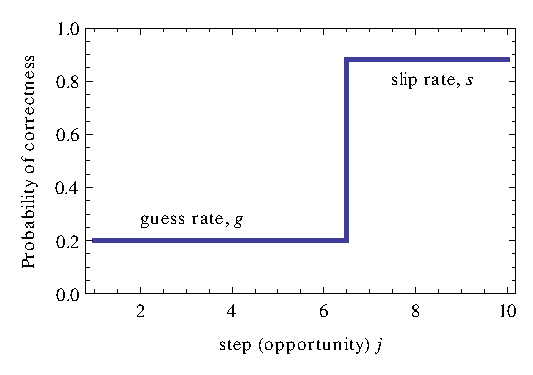
\includegraphics{step-model.eps}
  \caption{Functional form of the step model.}
         \label{stepf}
\end{figure}

In previous work, we introduced a simple ``step model'' of learning
and showed that it was competative with other common models
of learning, when applied to individual student 
data~\cite{van_de_sande_applying_2013}.
It is the simplest possible model where learning occurs at
a definite time and contains the guess and slip rates of Corbett and 
Anderson~\cite{corbett_knowledge_1995}.  It is defined as:
%
\begin{equation}
               P_\mathrm{step}(j) = \left\{\begin{array}{cc}
                                       g,& j<L\\
				       1-s,& j\ge L
                                    \end{array}\right. \label{step}
\end{equation}
%
where $g$ is the guess rate, $s$ is the slip rate and 
$L$ is ``the moment of learning,'' the step where the student
first shows mastery of the KC; see Figure~\ref{stepf}.  The case $L=1$
corresponds to no learning and $g$ is ignored.
%
We can fit $P_\mathrm{step}(j)$ to the student data using the
Maximum Likelihood method and determine maximum likelihood estmators
for the model parameters.  

Since the maximum likelihood estimator for $L$ often has large
uncertainties, it is useful to consider the model for each value of $L$
to be a separate ``sub-model''  $P_{\mathrm{step},L}(j)$ with parameters
$s$ and $g$.
Thus, for a given $L$, we can define the performance gain,
%
\begin{equation}
     % need actual formula here.
         \Delta_L = 1- \hat{g}+\hat{s}\; .
\end{equation}
%
where $\hat{g}$ and $\hat{s}$ are the
Maximum Likelihood estimators for $g$ and $s$ given by submodel
$P_{\mathrm{step},L}(j)$.
This allows us to use a multimodel approach~\cite{burnham_model_2002}.
Each sub-mode $P_{\mathrm{step},L}(j)$ has a relative probability given 
by its Akaike weight,  
%
\begin{equation}
                   w_L = \frac{\mathrm{e}^{\mathcal{L}_L-2}}{W}\, ,
\end{equation}
%
with normalization $W$ such that $\sum_L w_L=1$.


\section{Study 1}

UW Platteville, 111 students, 132 hours of student data, winter of 2012.  
Tutor randomly chooses policy: 
\begin{enumerate} 
\item After error, give unsolicited hint or not?
\item Give normal hint sequence or give bottom-out hint first?  
\end{enumerate}

\section{Objective function}

The basic approach for solving this problem, in terms of reinforcement
learning, is called a ``direct policy search.''
For each student, help-giving policy, and KC, we define the objective 
function to be 
%
\begin{subequations}
  \label{objective}
  \begin{align}
  Z =& \sum_L w_L \left\{\sum_{j \in \mathcal{I},\,j<L}  
  % Actually, we use the number of incorrect steps
  % between j and L for the discount factor.
  % need to add this to formula.
       \frac{\gamma^{n(j,L)} \Delta_L}{\left|\sigma_j\right|}
  \sum_{k\in \sigma_j} \left(f(\mathbf{x}_k)-d_k\right))^2 \right.
     \label{before} \\
 % reward for after-learning policy
 % Includes case with no learning as k=0.
  &+\beta \left. \sum_{j \in \mathcal{I},\,j \ge L} \frac{1-\hat{s}}
      {n(L,j_\mathrm{max})\left|\sigma_j\right|}
             \sum_{k\in \sigma_j} \left(f(\mathbf{x}_k)-d_k\right))^2
     \right\}
  \label{after}
  \end{align}
\end{subequations}
%
where $L$ labels different models, each with weight $w_L$;
$\mathcal{I}$ is the set of steps associated
with that student, policy, and KC that were marked ``incorrect.''  
$\sigma_j$ is the set of transactions associated with step $j$,
$f(\mathbf{x}_k)$ is the machine-learned policy associated
with transaction $k$ and
$d_k\in \{0,1\}$ is the
policy actually taken by the random-help version of Andes for that 
transaction.
We have arranged things so that finding an optimal policy 
corresponds to {\em minimizing} $Z$.

The first term (\ref{before}) rewards policies applied directly before
the moment of learning (or step $j=L$ for model $L$).  
These are weighted by the 
average performance gain $\Delta_L = 1-\left\langle g+s\right\rangle_L$ 
predicted by model $L$.
Also, $n(j,L)$ is the number
of incorrect steps $\mathcal{I}$ between $j$ and $L$, 
and $\gamma$ is the ``discount factor''~\cite{russell_artificial_2002}. 
A good value for $\gamma \in [0,1]$ must be determined empirically.
In a previous study involving physics learning~\cite{chi_empirically_2011}, 
$\gamma=0.9$ was chosen.
However, in that case, the discount factor was applied transaction-wise in 
a situation where there were many transactions per step.  In our case, 
we apply $\gamma$ step-wise to incorrect steps $\mathcal{I}$, 
suggesting a lower number might be appropriate.

Also, the tutor must have a strategy to apply in the case of slips: 
errors that occur after the student has learned the KC.
The second term (\ref{after}) rewards policies applied after
the KC has been learned.  Since the only available measure of 
effectiveness after the moment of learning is the slip rate $\hat{s}$, 
we look for a policy that maximizes $1-\hat{s}$.  The reward for 
this policy is evenly divided among the $n(L,j_\mathrm{max})$ 
incorrect steps after $L$.
Since our primary objective is to produce learning in the first
place (\ref{before}), we want the contribution of (\ref{after})
to $Z$ to be somewhat smaller.  Thus, we choose $\beta$ numerically 
such that the contribution of (\ref{after}) is somewhat smaller than 
the contribution of (\ref{before}).

The machine learning algorithm finds a function $f$ that acts on
the set of states $\left\{\mathbf{x}_k\right\}$ that minimizes
the objective function $Z$ summed overs students and KC's.  
Since our policies are binary-valued
and many of our features are well ordered (times, counts of transactions,
{\em et cetera}), it is natural to define $f$ in terms of a 
linear classifier.  Thus
%
\begin{equation}
              f(\mathbf{x}_k) = \left\{\begin{array}{cc}
		1,& \mathbf{a}\cdot \mathbf{x}_k <b \\
                0, & \mathbf{a}\cdot \mathbf{x}_k \ge b
		\end{array} \right.
\end{equation}
%
That is, $\mathbf{a}$ and $b$ define a hyperplane in feature
space.  All states on one side of the plane are given policy 0
and states on the other side have policy 1.
Numerically, we find $\mathbf{a}$ and $b$ that minimizes $Z$
summed over students and KC's.

\section{Feature space}

The student state at any given time is described by a list of
features.   Since the machine learned policy is to act on this list of
features, they must be computable in real time.  This is can be a
challenge in tutor system with a free-form interface like  Andes:
there is not always a way to determine, in real time, what a student was
attempting when they make an entry and get it wrong, even if the attempt
is examined by an expert human tutor.  Andes has a
number of error handlers that do make such a determination, but they 
apply only for certain well-known errors.

For determining which features to select, we used Min Chi's thesis
as a starting point~\citeyear{chi_micro-level_2009}, 
although she was doing this for a
rather different kind of tutor system.  The following items were
chosen mostly for convenience, and they avoided issues with determing
the KC associated with an entry.
%
\begin{description}

\item[logSessionTime] Log of number of seconds since start of current
  session.  This is a measure of student fatigue.

\item[fracSessionFlounderTime] Flounder time is the time spent between 
incorrect (object turns red) transactions, with no intervening correct 
(object turns green) transactions. 
 {\em fracSessionFlounderTime} is the total flounder
time for the current session over total session time.

\item[logNowRedTrans] Log of number of transactions since last
  correct (object turns green) transaction.

\item[logNowRedTime] Log of number of seconds since last
  correct (object turns green) transaction.

\item[logNowIdleTime] Log of number of seconds since last transaction.

\item[sessionCorrect] Number of objects in current session that have
  been  been marked  correct.

\item[sessionIncorrect] Number of transactions in current session where 
   object has been marked  incorrect.

\item[sessionHelp] Number of help requests in current session.

\item[fracSessionCorrect] $\mbox{sessionCorrect}/\left(\mbox{sessionCorrect}+\mbox{sessionIncorrect}+\mbox{sessionHelp}\right)$.

\end{description}
%
We have taken the logarithm of quantities where the student data
for that quantity ranges over several orders of magnitude.

On the Andes help server, the state for a given transaction 
is determined before the student action itself is analyzed,
in order that the help policy for that transaction can be set.  
Thus the state can only depend correct/incorrect (or floundering) 
information from previous transactions. 

\section{Study 2}

Improved help version of Andes with dynamic calculation of student state; find machine learned hinting policy for that state; give help based on policy.


Run at St. Anselm College May-July 2012, 16 students, 387 total hours, 
for entire two-semester course.  


For each homework set, half of the students, chosen at random, were
assigned to the experimental condition and half were assigned to
the control condition.  Thus, the experimental design is a mixed 
factorial design.
This means that individual students sometimes switched
between the experimental and control conditions over the course of the
semester.  Thus, for any student-KC sequence that spans multiple
homework sets, the student may have learned the skill in either 
condition.  Since the Akaike weights  give us the probability that 
learning occurred at step $j$, we then can find the probability 
the learning occurred
during the experimental condition versus the control condition.


\section{Study 2 Results}
%
% Need to define \Delta and L and student-KC sequence.
%

\begin{figure}
   \centering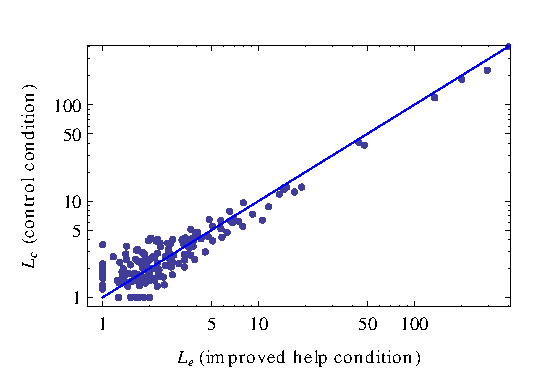
\includegraphics{scatter-step.eps}
   \caption{Scatter plot of the moment of learning $(L_e,L_c)$ for each
     KC, averaging over students.  If the experimental intervention causes
     faster learning then $L_e<L_c$ and more points would lie to the 
     left of the diagonal line.
     The weighted average over all KCs of $L_e-L_c = -0.05\pm 0.04$ ($p=0.12$).
     Although the value of $L$ varies widely as a function of KC, there
     is no large change in L across experimental condition.
   }\label{scatterstep}
\end{figure}

\begin{figure}
   \centering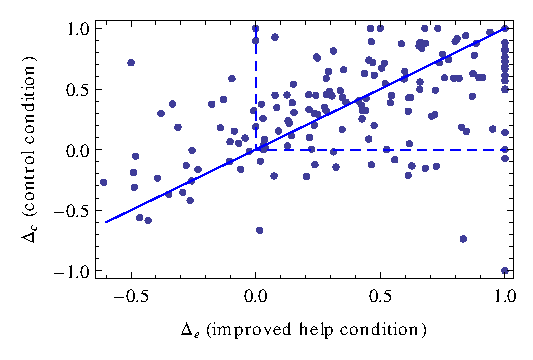
\includegraphics{scatter-gain.eps}
   \caption{Scatter plot of performance gains $\left(\Delta_e,\Delta_c\right)$
   for each KC, averaging over students.  If the experimental intervention
   causes greater learning then, $\Delta_e > \Delta_c$ and more points
   would lie to the right of the diagonal line.
 %  Individual data points have large 
 %  uncertainties (standard error of order 1).
   The weighed average over all KCs of $\Delta_e - \Delta_c = 
        0.008\pm 0.038$ ($p=0.41$).
   Note that there are a number
   of KCs with negative learning $\Delta<0$, probably due to 
   assignment problems that ramp quickly in complexity. 
   }\label{scattergain}
\end{figure}

We can also ask how much student improved in each experimental condition.
Thus, for each condition, we calculate, for each KC, 

\section{Conclusion}

Introduced method for iterative improvement of help-giving policies using 
{\em in situ} assessment.

Completed one cycle of iterative process:  need larger sample size.

Conjecture: inclusion of preemptive hints (hints before student attempts
a step) may be crucial for Andes. 

% Bibliography
\bibliographystyle{acmlarge}
\bibliography{education-modeling}

\end{document}